%\cleardoublepage
\pagenumbering{arabic}\setcounter{page}{1}
\chapter{INTRODUCTION}
\label{ch:Introduction}

%\section{Background}
%\label{sec:Intro:Background}

%	\subsection{A Brief History of Space Conditioning}
%	\label{subsec:Intro:Background:History}
%
%Space conditioning for human comfort is something that has been desired by mankind since early history. We know from the archaeological record that early man used fire prevalently to stay warm. Native American Indian tribes were also said to have settled near natural geothermal hot springs \citep{DOEHistory2012}. Little is known of early man's efforts to stay cool.
%
%Later in human history we know that the luxury of space cooling, based on the written record, has typically only been available to royalty and the elite. Early Chinese emperors are said to have used 10 ft.\ (3 m) diameter fans for space ventilation \citep{NeedhamLing2000}. These fans were manually or ``water" powered and imperial palaces were designed to promote natural air ventilation. Wealthy Romans were also said to have used their extensive water infrastructure for space cooling \citep{Slate2011}.  This is said to have been accomplished by passing cool water through the walls in their homes. 
%
%More recently, in the 19\textsuperscript{th} century, the ice trade was a major industry fueled by the people's demand for comfortable indoor environments \citep{Nagengast1999}. In 1864, George Knight \citep{Anonymous1921} proposed the first indoor hospital ventilation system. He proposed cooling space air by passing it through a cooling coil which was immersed in melting ice. For heating, the mid 1890's saw the birth of the United States' first district heating system \citep{IdahoRenewableEnergy2012} which was built in Boise, Idaho. This system piped hot geothermal water to over 200 businesses and homes to provided for space heating. It also provided hot water for the city's 65 ft.\ (20 m) by 125 ft.\ (38 m) indoor swimming pool.
%
%Advances in mechanical cooling and heating science and technology by Carnot, Thompson (Lord Kelvin), Gorrie, Carrier, and many others eventually led to the demise of the ice harvesting and distribution industry \citep{Gladstone1998}. Mechanical cooling eventually took over the space cooling market by the early 1920's \citep{Nagengast1999}. Additionally, over the last several decades, heating provided via mechanical means has also seen an increase in popularity as opposed to heating provided by electricity, or heating provided via wood, natural gas, propane, or heating oil combustion.

	\section{Current Challenges in Space Conditioning}
	\label{sec:Intro:Background:CurChallenges}

In this day and age, it is obvious that we wish to maintain a comfortable indoor environment. There are, however, other factors besides comfort that must be considered when looking at space conditioning systems. System performance, life cycle cost, and space requirements are just a few of the important aspects a designer will consider when selecting a heating or air-conditioning system. Another aspect of space conditioning system design that carries significant importance is environmental impact, which is directly related to system efficiency. Building owners, operators, and designers are increasing their awareness of building energy use and how it is affecting the environment around them. This is partially driven by rising energy costs, but also due to the fact that they generally desire to be good stewards of the energy their systems are using. Other programs and initiatives such as Energy Star, or Leadership in Energy and Environmental Design (LEED) have helped push ``green" building and energy efficient design to the forefront of the building sciences.

In 2010, residential and commercial buildings used 41.1\% of primary energy consumption in the United States. This was greater than all of industrial energy use (30.8\%) or transportation energy use (28.1\%) \citep{DOE2010}. From those statistics, it should be fairly obvious that the energy consumed to maintain a comfortable indoor environment is significant. Even small changes in system efficiency and energy use will result in significant cost and environmental impacts.

\section{Surface Water Cooling and Surface Water Heat Pump Systems}
\label{sec:Intro:SystemOverview}

As a result of the ``green" building movement, system designers are continuously looking for ways to make their designs more energy efficient, and thereby more environmentally friendly. One technology that is gaining acceptance in the built environment community is the use of surface water cooling or surface water heat pump systems. Surface water cooling or surface water heat pump systems are similar to geothermal heat pump systems in that they can use the earth's naturally occurring heat (or lack thereof) to meet heating or cooling loads. What makes these systems so attractive is that they can achieve very high levels of energy efficiency. In this study, `geothermal energy' is defined as low enthalpy geothermal energy.

Surface water cooling (SWC) systems are systems that take cold water from a surface water body, i.e. ocean, lake, pond, or river, and dissipate the building's cooling load to the surface water. Surface water heat pump (SWHP) systems can dissipate heat from the building cooling load to surface water, but they can also extract heat from the surface water to satisfy a building heating load.

SWC and SWHP systems can be broken down into two main categories: open-loop systems and closed-loop systems. This section will describe the basic operation of each system type.
	
	\subsection{Open-loop Systems}
	\label{subsec:Intro:SystemOverview:OpenLoop}

		\subsubsection{Open-loop Surface Water Cooling Systems}
		
Open-loop SWC systems take cold water from surface water bodies and use that water to meet a cooling load which can be seen in Figure \ref{fig:Intro:SystemOverview:OpenLoop:OLDirectCooling}. Here, we can see that cold water is taken from a surface water body and is piped into a wet sump pit. From there it is taken and pumped through an isolation heat exchanger who's purpose is to isolate the potentially contaminated open-loop from the closed circulation loop. At the isolation heat exchanger, the cold water taken from the surface water body exchanges heat with the closed loop circulation system that directly meets the cooling load. Once the surface water passes through the isolation heat exchanger, it is then returned at a warmer temperature back to the surface water body.

	\begin{figure}
		\centering
		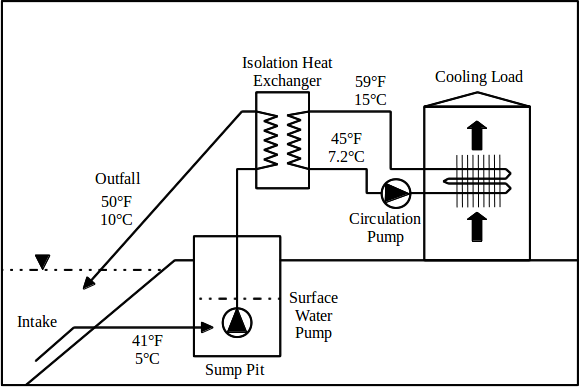
\includegraphics[width=0.8\textwidth]{OL_Direct_Cooling.png}
		\caption[Open-loop direct surface water cooling system]{Open-loop direct surface water cooling system}
		\label{fig:Intro:SystemOverview:OpenLoop:OLDirectCooling}
	\end{figure}

The most prominent advantage of an open-loop SWC system is that no mechanical cooling equipment is required. This allows these systems to operate at exceptionally high values of system COP; system COP values above 25 have been reported \citep{Peer2012} for very large (20,000 ton (70.3 MW)) systems. The primary energy consumers are the circulation pumps and optimal system design depends heavily on intake piping and pumping design.

Open-loop SWC systems are, however, limited by the fact that they require cold surface water that is naturally occurring. Typical locations where this technology may be feasible are near the shores of deep lakes or oceans. An ideal location would be a deep lake or ocean with a steep shoreline bathymetry. This would allow for the placement of an intake pipeline that is as short as possible. Since the intake pipeline is anticipated to be 50-85\% of the total system cost (\cite{Ciani1978} and \cite{LeraandVanRyzin1995}), shorter intake pipelines will result in lower overall initial cost. 

Another system limitation is the requirement that the system entering water temperature be sufficiently cold so that the load may be met. In order to meet the dehumidification requirements of a building cooling load, \cite{Ciani1978} states that system entering water temperature should be $50^\circ \mbox{F}$ ($10^\circ \mbox{C}$) or lower. \cite{KavanaughPezent1990} state that surface water can be used for direct cooling with surface water temperatures up to $55^\circ \mbox{F}$ ($12.8^\circ \mbox{C}$).  Some sensible cooling can be accomplished with the use of warmer system entering water, but satisfying the latent dehumidification load may require other means.

		\subsubsection{Open-loop Surface Water Heat Pump Systems}

Open-loop SWHP systems can meet a cooling load, however they also have the advantage that they can meet a heating load if designed properly and equipped with a reversible heat pump. An example of an open-loop SWHP system operating in cooling mode can be seen in Figure \ref{fig:Intro:SystemOverview:OpenLoop:OLHeatPumpCooling}. Similar to the SWC system, the open-loop SWHP system takes water from a body of surface water and passes it through an isolation heat exchanger. This water then exchanges heat with a closed circulation loop which will then exchange heat with either the evaporator or condenser of a reversible heat pump. The heat pump then cools or heats another closed circulation loop that will then directly meet the heating or cooling load. Because the heat pump can operate in heating or cooling mode, the water returning to the surface water body can be warmer or cooler that it was originally.

	\begin{figure}
		\centering
		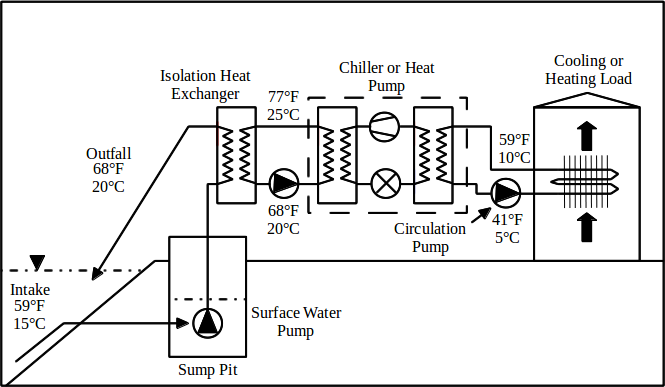
\includegraphics[width=0.8\textwidth]{OL_HP_Cooling.png}
		\caption[Open-loop surface water heat pump system]{Open-loop surface water heat pump system}
		\label{fig:Intro:SystemOverview:OpenLoop:OLHeatPumpCooling}
	\end{figure}

The primary advantage of an open-loop SWHP system is that meeting the cooling or heating load is less dependent on the conditions of the surface water. If the system entering water temperature is greater than what is required to meet the latent or sensible cooling load, the heat pump can make up the difference and allow the load to be met. Open-loop heat pump systems also do not have to overcome surface water heat exchanger thermal resistance. This can allow for system COP to be better than closed-loop systems.

The first disadvantage of an open-loop SWHP when compared to a open-loop SWC system is the initial cost of the heat pump. For very large systems, this cost will be significant, however, because the system is less dependent on entering system water conditions, the cost of the intake pipeline may be reduced thus offsetting the overall project cost. Another obvious disadvantage of this system type is the additional energy that must be consumed by the heat pump and additional circulation pump.

There are currently no studies that compare the life cycle costs of open-loop SWC or SWHP systems relative to more conventional cooling systems, such as a system with a chiller coupled with an evaporative cooling tower to meet the cooling load and a natural gas boiler to meet the heating load. More work in this topic area would be useful.

	\subsection{Closed-loop Systems}
	\label{subsec:Intro:SystemOverview:ClosedLoop}

		\subsubsection{Closed-loop Surface Water Cooling Systems}

Closed-loop SWC systems function in a manner very similar to the open-loop SWC system that is indicated in Figure \ref{fig:Intro:SystemOverview:OpenLoop:OLDirectCooling}. Water or an anti-freeze solution is circulated between an isolation heat exchanger and a surface water heat exchanger (SWHE) that is submerged in a nearby surface water body. At the isolation heat exchanger, the two closed circulation loops can exchange heat to meet the cooling load. The now warmer surface water loop is then recirculated back to the SWHE where it can reject heat to the source water body.

Closed-loop SWC systems are uncommon. In fact, this author is only conscious of one instance where a hybrid closed-loop surface water cooling/surface water heat pump system has been installed. \cite{Lockhart2013} stated that he had installed a system on a 15,000 $\mbox{ft}^2$ (1,394 $\mbox{m}^2$) private residence near Victoria, Canada. This system could be operated in direct cooling mode during summer months or in surface water heat pump mode for heating in winter months. \cite{Lockhart2013} stated that summer seawater temperatures along the Pacific coast near Victoria Canada are around 52$^\circ \mbox{F}$ (11$^\circ \mbox{C}$) during the summer months. At those temperatures, a good deal of space cooling can be accomplished. The system discussed was coupled to an in-floor hydronic system, and therefore no latent or dehumidification load could be satisfied by the system.
	
		\subsubsection{Closed-loop Surface Water Heat Pump Systems}	
	
Closed-loop SWHP systems function very similar to open-loop SWHP systems, except that the isolation heat exchanger and open-loop intake system are replaced by a closed circulation loop and surface water heat exchangers. Water or anti-freeze solution circulates between the SWHE and the heat pump. The heat pump can then either accept heat from, or reject heat to the surface water loop based on the mode of operation. The heat pump can be a water-air heat pump and directly heat or cool the building space air, or it can be a water-water heat pump as indicated in Figure \ref{fig:Intro:SystemOverview:ClosedLoop:CLSWHPsystem}, which  shows a schematic of a closed-loop SWHP system. By using a water-water heat pump, a single heat pump unit could provide heating or cooling to multiple zones.

	\begin{figure}
		\centering
		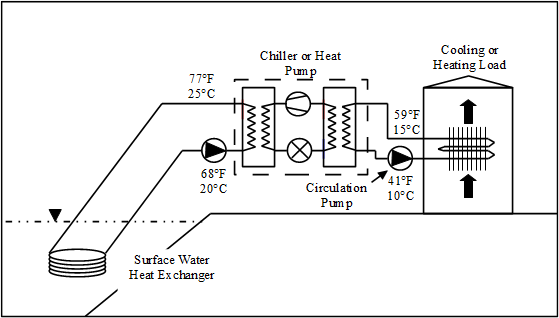
\includegraphics[width=0.8\textwidth]{CL_HP_Cooling.png}
		\caption[Closed-loop surface water heat pump system]{Closed-loop surface water heat pump system}
		\label{fig:Intro:SystemOverview:ClosedLoop:CLSWHPsystem}
	\end{figure}	

An advantage of closed-loop SWHP systems is that they can operate in bodies of source water where the source water quality may be low. Open-loop system often require screening to prevent fish or other debris from being entrained into the intake, however, since the closed loop system doesn't directly circulate the source water, there are no screening requirements. They can also be operated in locations where the elevation difference, and thus, static head between the source water and the heat pump system is significant. Open-loop surface water pumps must be at or below source water body level in order to satisfy the net positive suction head requirements of the pump. If pump's required net positive suction head exceeds intake pipeline's available net positive suction head, cavitation will occur at the pump inlet. Closed-loop systems do not require the pump be near the elevation of the source water body. Thus, greater elevation differences between heat pump system and source water level are possible.

Another important advantage of closed-loop SWHP systems when compared to open-loop SWHP systems is that they can operate with surface water loop temperatures at or below the freezing point of pure water. When the system is operated in heating mode, the system is extracting heat from the source water body. To do this, the heat pump must lower the surface water loop temperature below the temperature of the source water body. Often during winter months, surface water temperatures can approach freezing conditions (\cite{KavanaughRafferty1997} and \cite{Selvakumar2013}), especially in northern latitudes, which may cause loop temperatures to drop below the freezing point of pure water. In these applications, an anti-freeze solution is used as the heat transfer fluid in the surface water loop in anticipation of this. 

\section{Surface Water Heat Exchanger Overview}
\label{sec:Intro:HXOverview}

There are numerous surface water heat exchanger designs that have been developed over the years. Spiral-helical, plate, capillary, slinky, and embedded type heat exchangers is a short list surface water heat exchanger types. This study will focus primarily on spiral-helical heat exchangers with a brief description of plate heat exchangers.
	
	\subsection{Spiral-helical Heat Exchanger}
	\label{subsec:Intro:HXOverview:SpHelHX}
	
Spiral-helical heat exchangers are a common heat exchanger type used for closed-loop SWHP systems. This is because they are typically constructed from HDPE pipeing which is an inherently inexpensive construction material. A picture of a spiral-helical SWHE can be seen in Figure \ref{fig:Intro:HXOverview:SpHelHX:SWHEPic}. A central hub along with horizontal and vertical tube-tube spacers can also be seen in Figure \ref{fig:Intro:HXOverview:SpHelHX:SWHEPic}. The central hub is a jig that was built for the purpose of building spiral-helical SWHEs \citep{Hansen2011}.

	\begin{figure}
		\centering
		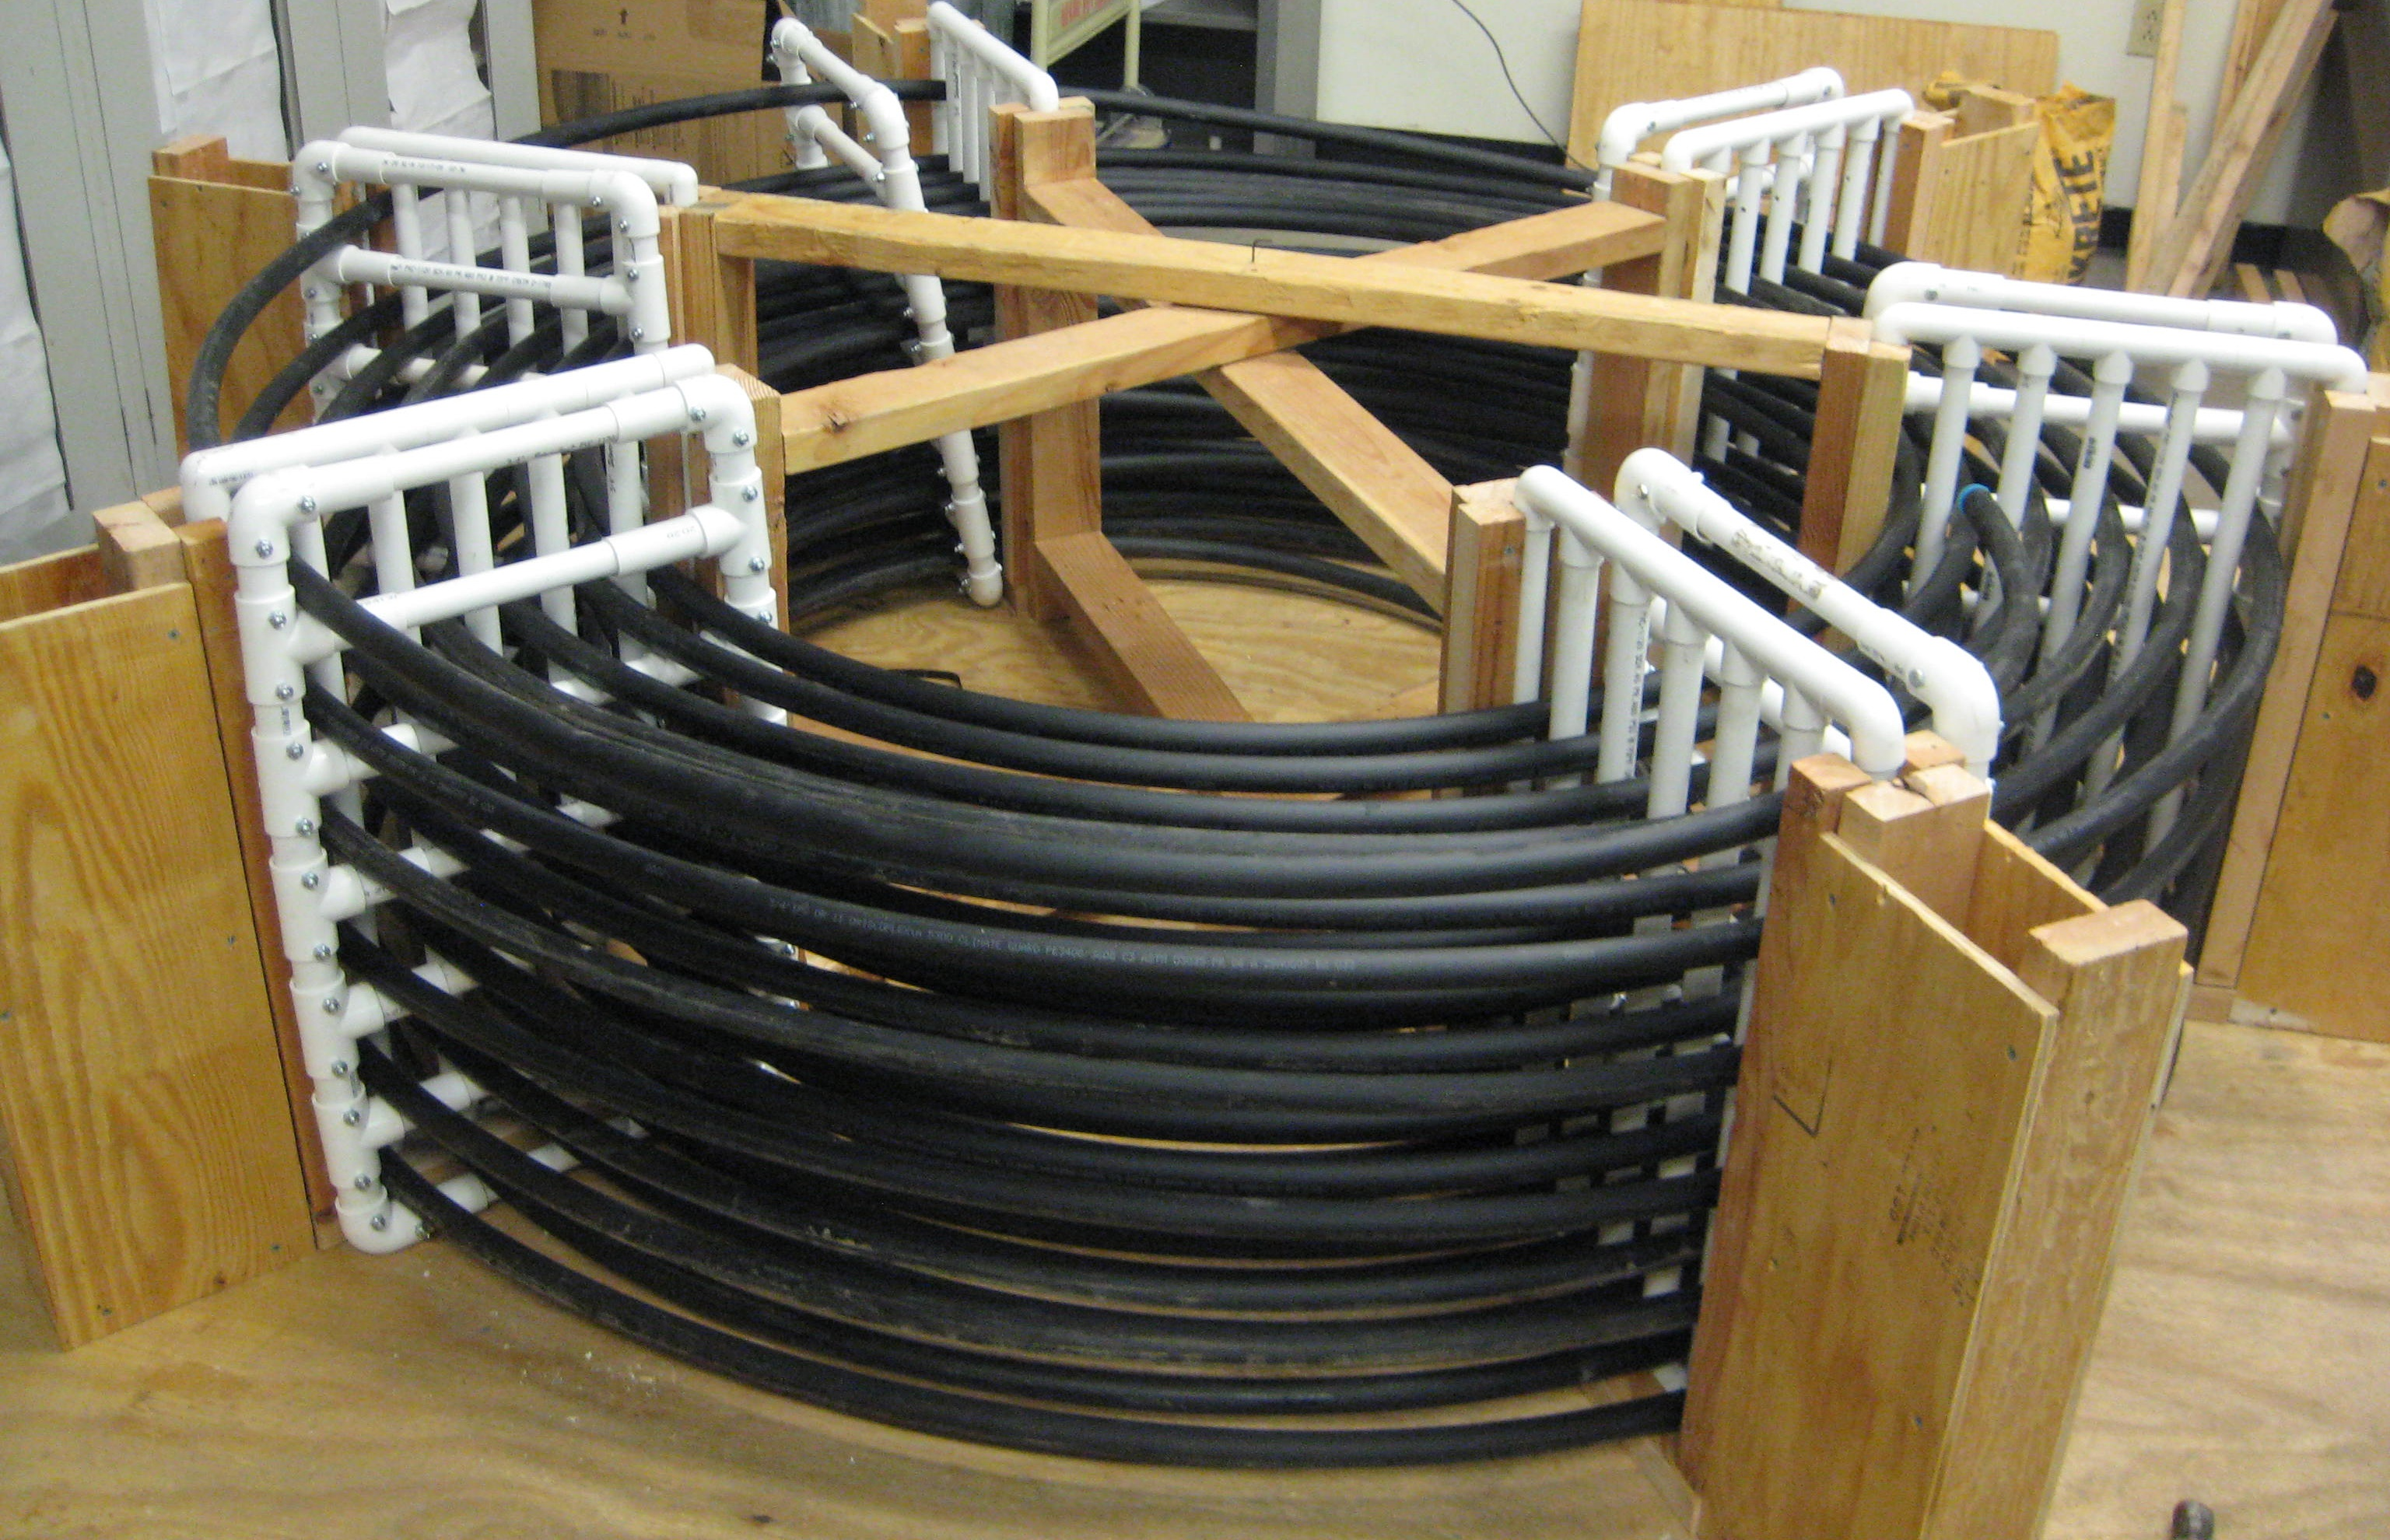
\includegraphics[width=0.8\textwidth]{SWHE_Pic.jpg}
		\caption[Spiral-helical heat exchanger]{Photo of spiral-helical heat exchanger.\textit{Reprinted, by permission, from \cite{Hansen2011}}}
		\label{fig:Intro:HXOverview:SpHelHX:SWHEPic}
	\end{figure}	
	
%	\begin{minipage}{.5\linewidth}
%    Foo\footnote{bar}
%	\end{minipage}

Spiral-helical heat exchangers are constructed from straight HDPE tubing which then is formed into a coil. HDPE tubing lengths range typically from 300-500 ft.\ (91-152 m) in length. One way to form a spiral-helical coil is to begin by positioning horizontal tube spacers around a central hub. The straight tube is then taken and wrapped around the hub beginning at the center, and then wrapped outward in a spiral fashion until tubing is placed between all horizontal tube spacers. A row of vertical tube-tube spacers is then placed on top of the first horizontal ``spiral" layer. The tubing is then taken upward one level in a ``helical" fashion. The tubing is then wrapped back toward the center of the coil until the horizontal tube-tube spacers are full again and another ``spiral" layer is completed. This is process is then repeated until the coil is constructed. Figure \ref{fig:Intro:HXOverview:SpHelHX:SWHESchematic} shows a schematic of the spiral-helical SWHE. The section view of Figure \ref{fig:Intro:HXOverview:SpHelHX:SWHESchematic} shows the consecutive tube numbers based on when they were placed in the coil. Also shown are the SWHE inside and outside diameters.
	
	\begin{figure}
		\centering		
		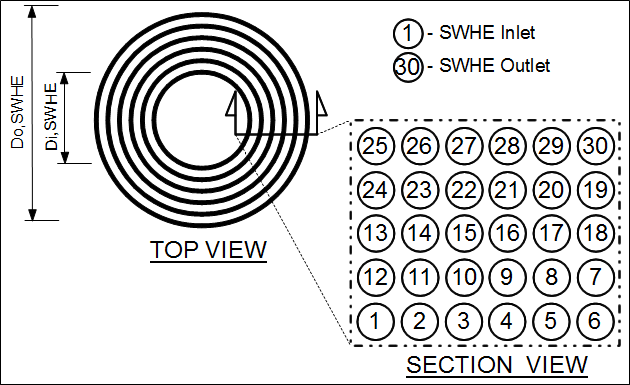
\includegraphics[width=0.8\textwidth]{SWHE_Schematic.png}
		\caption[Schematic of spiral-helical heat exchanger]{Schematic of spiral-helical heat exchanger}			
		\label{fig:Intro:HXOverview:SpHelHX:SWHESchematic}
	\end{figure}
	
	
	\subsection{Plate Heat Exchanger}
	\label{subsec:Intro:HXOverview:PHX}
	
Plate type heat exchanges are also a very popular surface water heat exchanger type. Plate heat exchangers are typically constructed from stainless steel and they are placed vertically in the source water body. A 4 ft.\ x 5 ft.\ (1.2 m x 1.5 m), 4-pass, stainless steel plate heat exchanger can be seen in Figure \ref{fig:Intro:HXOverview:PHX:PHXpicture}. Also visible in Figure \ref{fig:Intro:HXOverview:PHX:PHXpicture} are the small indents made through out the plate. These small indents are places where the two sides of the plate have been welded together. This helps maintain turbulent flow on the inside of the plate.

	\begin{figure}
		\centering
		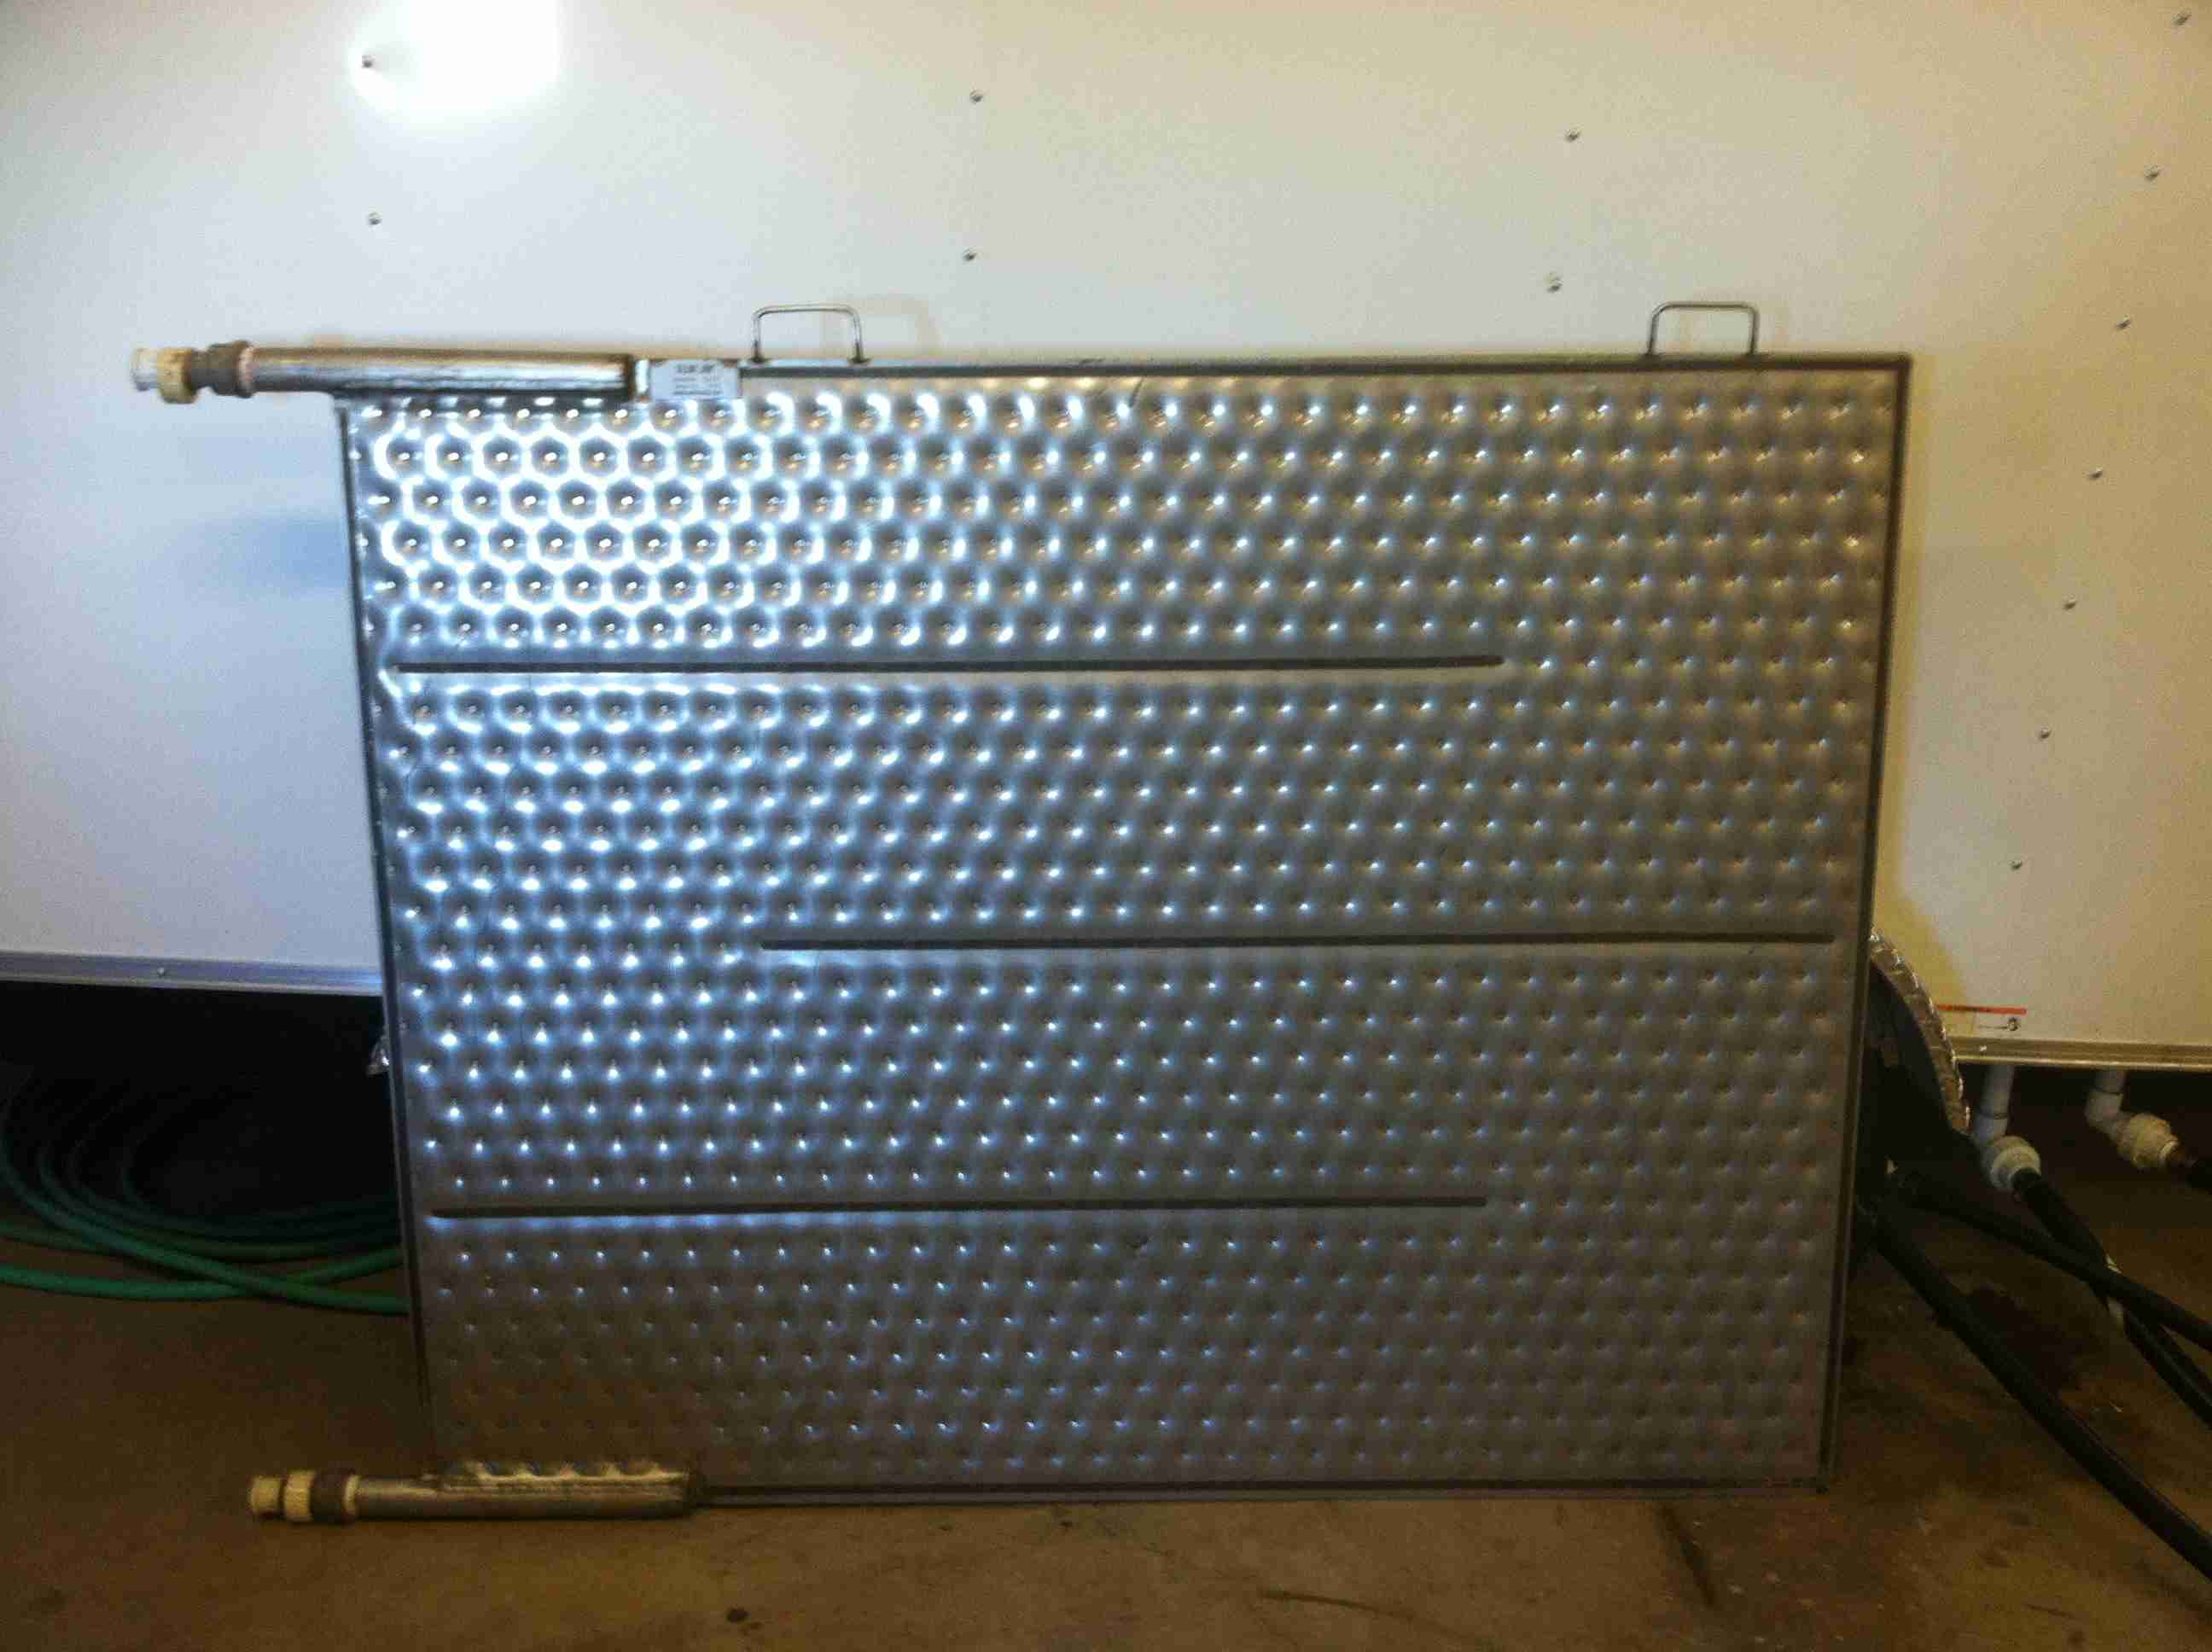
\includegraphics[width=0.8\textwidth]{Plate_HX.jpg}
		\caption[Stainless steel plate heat exchanger]{Stainless steel plate heat exchanger}
		\label{fig:Intro:HXOverview:PHX:PHXpicture}
	\end{figure}

Plate heat exchangers are often times the more popular heat exchanger type for larger commercial applications. The intensive labor involved with the construction and placement of spiral-helical, slinky, or other non-rigid type heat exchangers makes plate heat exchangers more attractive to SWHP system installers. This is because they can be arranged together relatively quickly into an array, attached to a frame, and lowered into position via crane. These frames also can keep the plate heat exchanger array elevated above the sediment at the bottom of the water source. Several plate heat exchanger arrays can be seen in Figure \ref{fig:Intro:HXOverview:PHX:PHXarray}. A plate heat exchanger array can also be seen lifted into place via crane in Figure \ref{fig:Intro:HXOverview:PHX:PHXcrane}.

	\begin{figure}
		\centering
		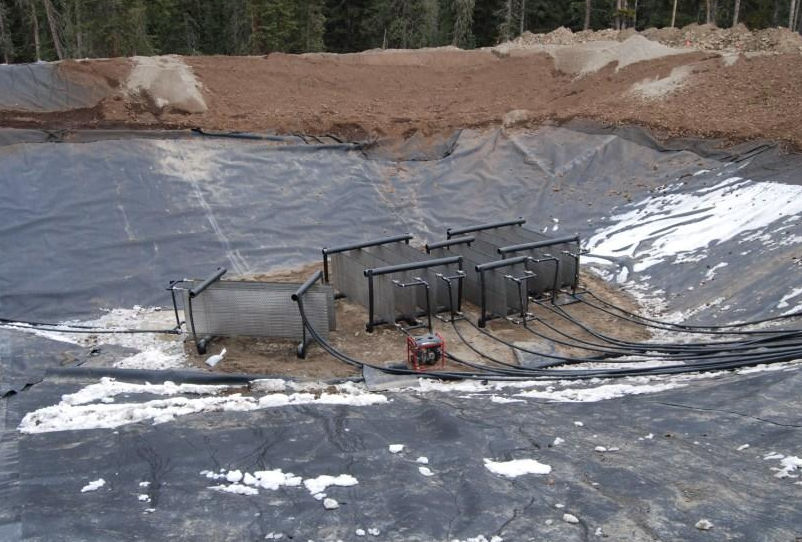
\includegraphics[width=0.8\textwidth]{Plate_HX_Array.png}
		\caption[Installed plate heat exchanger arrays]{Plate heat exchanger arrays for home  in Big Sky, MT. \textit{Reprinted, by permission, from Terry Proffer}}
		\label{fig:Intro:HXOverview:PHX:PHXarray}
	\end{figure}
	
	\begin{figure}
		\centering
		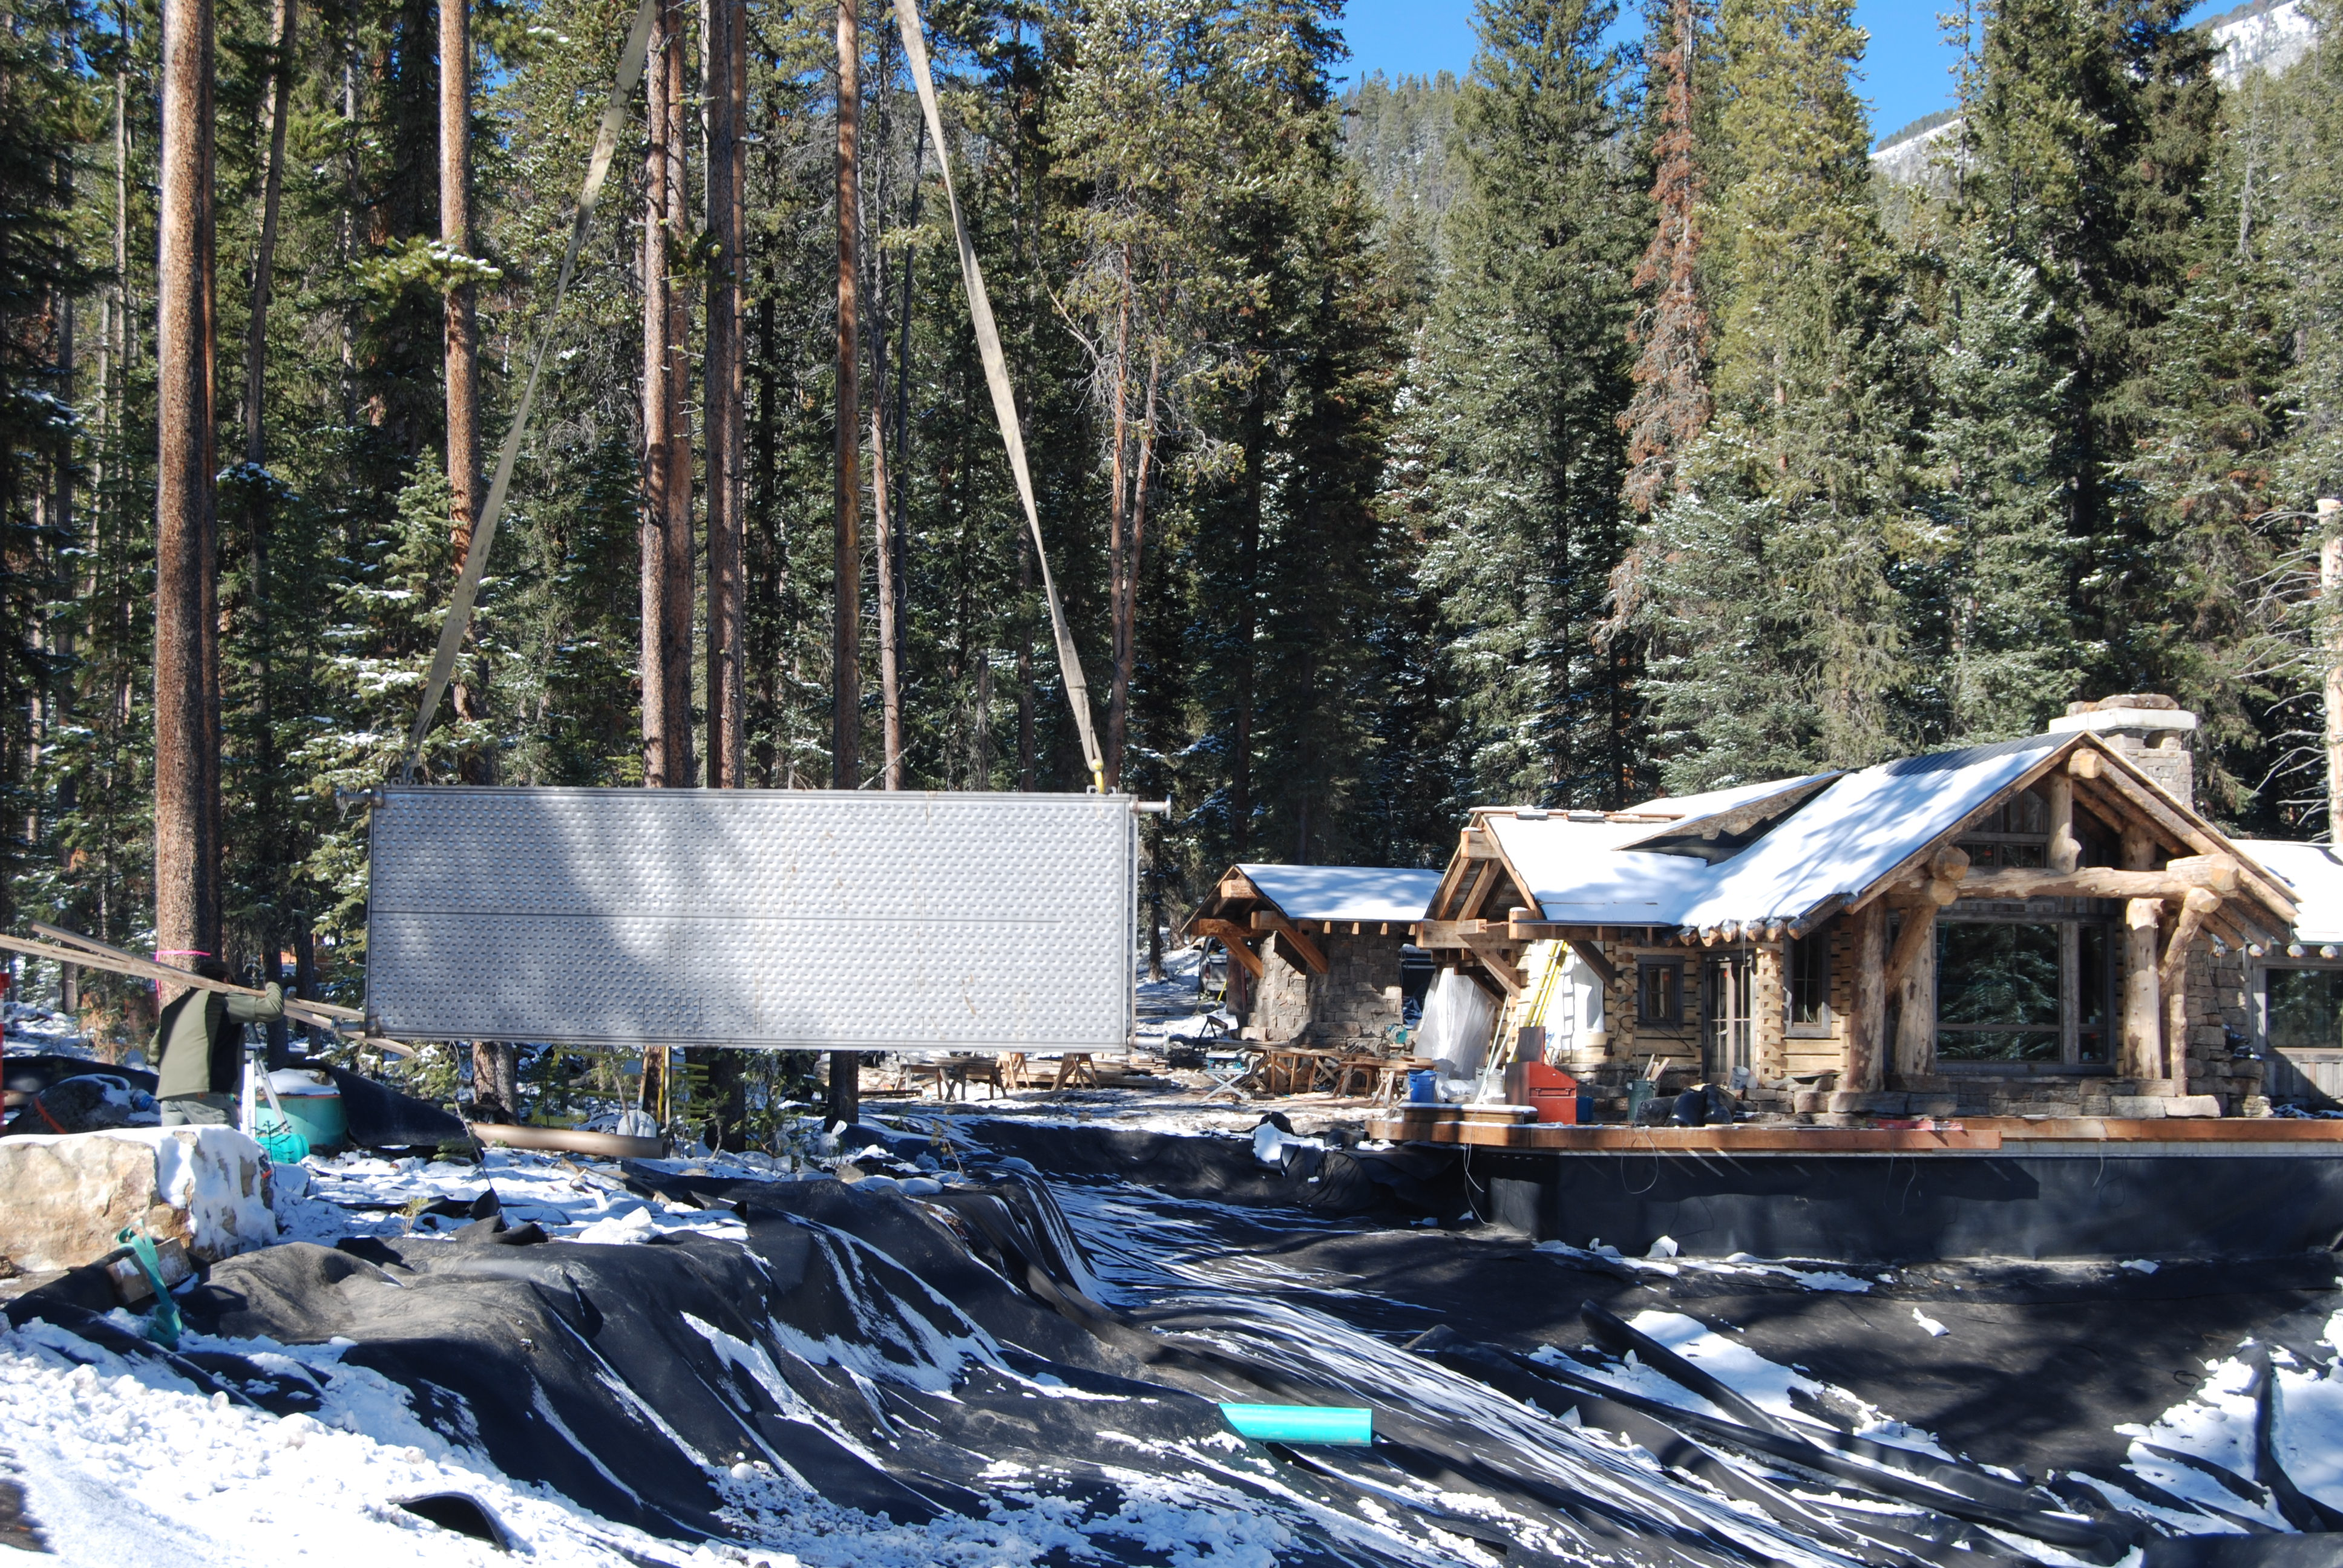
\includegraphics[width=0.8\textwidth]{Plate_HX_Crane.jpg}
		\caption[Plate heat exchanger array installation]{Plate heat exchanger array being lifted into place with a crane. \textit{Reprinted, by permission, from Terry Proffer}}
		\label{fig:Intro:HXOverview:PHX:PHXcrane}
	\end{figure}

\section{Literature Review}
\label{sec:LitRev}

	\subsection{Open-loop Systems}
	\label{subsec:Intro:LitRev:OpenLoop}

A journal article entitled: ``Open-loop Surface Water Cooling and Surface Water Heat Pump Systems -- A Review" was co-authored by the current author and published in the February 2013 issue of HVAC\&R Research \citep{MitchellSpitler2013}. In addition to what was covered in section \ref{sec:Intro:SystemOverview}, a few other notable points are:
	
\cite{Sumner1948} described the first known open-loop surface water heat pump system used for space conditioning. This system used the River Wensum in the UK as the source water body. During the winter of 1945-46 it is said to have obtained a COP of $3.45$ and provide a heating capacity of 800 MBTUh. It is unknown if the COP value is a system wide COP or a heat pump COP.

Since then, a variety of surface water cooling and surface water heat pump systems have been designed and constructed. In the year 2000, Cornell University began using direct surface water cooling to provide cooling for their entire campus \citep{PeerJoyce2002}. This system is capable of pumping 32,000 gpm (7,268 $m^3/hr$) from 250 ft.\ (76 m) beneath Lake Cayuga to provide up to 20,000 tons (70.3 MW) of peak cooling capacity. In 2010, the system COP was stated to be 25.8 \citep{Peer2012}.

In the early 2000s, the City of Toronto in Ontario Canada completed work on a very large hybrid SWHP system \citep{Heffernan2001}. The systems draws water from Lake Ontario at a temperature of $41^\circ$F ($5^\circ$C). The water is then filtered and treated to be used as the city's potable water and sent to a heat exchange facility. There, the treated lake water exchanges heat with the closed loop chilled water distribution system. The direct surface water cooling portion of the system alone is capable of producing 40,000 tons (141 MW) cooling capacity. Bottoming chillers can then reduce the plant supply water temperature to $38^\circ$F ($3.3^\circ$C) to give the system an additional 16,500 tons (58 MW) of cooling capacity \citep{Eliadis2003}. 

Additional information pertaining to pipeline, surface water pump, and heat exchanger design and material selection can be found treated in greater detail in  \cite{MitchellSpitler2013}.

	\subsection{Closed-loop Systems}
	\label{subsec:Intro:LitRev:ClosedLoop}
	
Prior to this work, there has been some information presented regarding the performance and design of closed-loop surface water heat pump systems, however, most of the information published was written in Swedish which limits its accessibility. Other information published in English by other authors is generally limited to handbook style design diagrams and is lacking in information which would be required for detailed calculations. A few of these works are summarized here. 
	
\cite{Backlund1982} described a system where 11 pieces of 164 ft.\ (50 m) long straight HDPE pipe with  an outside diameter of 1.6 in.\ (40 mm) and a wall thickness 0.1 in.\ (2.5 mm) were connected together in parallel. The system was designed to extract heat from the lake bed to provide for space heating. This was done by capping the ends of a smaller diameter (OD 1.2 in.\ (28 mm)) tube, and then placing it inside of the larger tube. Because the inner tube is filled with air, it was buoyant therefore floated to the top of the inner surface of the larger pipe. The heat transfer fluid was then circulated in the interstitial space between the tubes with the intent of enhancing heat transfer from the pond bottom. The design was based on a heat extraction rate of 31-52 BTU/hr-ft (30-50 $W/m$). Some anecdotal information was given regarding the placement of the tubes. The author stated that placing the tubes on the bottom creates less interference opportunities for fish, boats, currents, ice, etc. No system performance information is given.

\cite{SvenssonSorman1982} performed heat extraction experiments in a 32 in.\ (80 cm) deep pool using 1-1/2 in.\ (40 mm) HDPE tubing. The project's objective was to determine the heat transfer rate from the surrounding water and lake bottom material as a function of circulating fluid temperature. The experiments were performed in 32-39$^\circ$F (0-4$^\circ$C) stagnant water with varying mixtures of sand and organic-rich sediments to mimic natural lake bottom materials. Various degrees of pipe embedment into the base materials were also tested. An extensive theoretical discussion is given and the experimental results are presented as a series plots and charts for each different condition. Ice fouling of heat exchanger tubing is also discussed.

\cite{SvennsonSorman1983} performed a series of laboratory experiments on tubes placed in running water for heat uptake. An experiment was designed so that the angle between the tube axis and flow direction could be varied. Surface water flow velocity and temperature were also varied. The results were presented in a series of design graphs indicating the heat exchanger performance. The authors also presented experimentally derived outside Nusselt number correlations. The authors concluded that tube-tube spacing can be fairly narrow given that the surface water flow velocity is greater than 10 ft/min (5 cm/min). At slower flow velocities, tube-tube spacing should be expanded to 10-20 in.\ (25-51 cm).

A great amount of work relating to surface water heat pump systems can be found in \cite{BFRseminar1982}, which is a compilation of conference papers presented in 1982. Here, a good deal of Swedish research from the period regarding surface water heat pump systems is compiled and summarized.
	
\cite{Kavanaugh1991} presents some information regarding the design of surface water heat pump systems. The author discusses open and closed-loop systems. Seasonal lake behavior is briefly discussed as well as various coil designs. Also presented are several design diagrams that give required coil length in ft/ton as a function of the temperature drop across the coil. The author does not specify whether the design heat transfer rate indicated in the plots is the coil heat transfer rate or whether it is the space heat transfer rate.

\cite{KavanaughRafferty1997} present what is likely the most comprehensive resource for surface water heat pump system design prior to the publication of \cite{Hansen2011}. Here, the authors briefly discuss seasonal lake temperature behavior. Several coil designs are presented and design graphs are presented which show required coil length in ft/ton as a function of approach temperature. Approach temperature is defined as the coil exiting fluid temperature minus the lake temperature. It is not stated whether the indicated heat transfer rate is a coil heat transfer rate or a space heat transfer rate. This approach also assumes that SWHP coils will perform equally at equal approach temperatures, regardless of lake temperature.

\cite{Hansen2011} presents a comprehensive review of SWHP systems, surface water heat exchangers, and presents the most current information regarding these systems to date. The author performed testing on SWHP systems with a specific focus on determining performance of various types of SWHEs. The author provided a review of inside and outside convection correlations for SWHEs. From which, he recommended the correlation developed by \cite{RogersMayhew1964} for determining inside convection resistance. He also determined that there were no external convection correlations which were suitable for modeling of spiral-helical SWHE. In order to develop a suitable correlation, the author updated the experiment developed by \cite{Austin1998} for SWHE testing. Several different varieties of surface water heat exchangers were tested. Specific to this work, the author \citep{Hansen2011} performed 528 heat rejection tests on spiral-helical SWHEs. From these tests, he developed an external convection correlation specific to spiral-helical SWHEs which is shown in Equation \ref{eq:Intro:LitRev:ClosedLoop:Hansen}.

	\begin{equation}
		\mbox{Nu}_{D,o} = 0.016 \, \mbox{Ra}_{D,o}^{* \, 0.264} \left(\frac{\Delta y}{D_o}\right)^{0.078} \left(\frac{\Delta x}{D_o}\right)^{0.223}
		\label{eq:Intro:LitRev:ClosedLoop:Hansen}
	\end{equation}
	
From this, he developed several design diagram for sizing SWHE under heat rejection conditions. Design diagrams for different surface water heat exchager designs were also developed and presented. All work was performed under space cooling, or heat rejection conditions.

\section{Scope of Study}
\label{sec:Intro:Scope}

The work conducted by \cite{Hansen2011} was taken as a starting point for this work because both projects were funded under the same ASHRAE research grant, RP-1385. Because of the continuous nature of the research, this study aims to bridge some of the remaining information gaps for surface water heat pump systems. 

In this study, experimental testing was performed on spiral-helical surface water heat exchangers. Several spiral-helical heat exchanger geometries were tested under heat rejection conditions. These tests were used to augment the \cite{Hansen2011} data set for heat rejection conditions. From there a space heating, or heat extraction, experiment was then constructed with the intent of determining spiral-helical SWHE performance under heat extraction conditions.

From these experiments, the convection correlation shown in Equation \ref{eq:Intro:LitRev:ClosedLoop:Hansen} was updated based on the additional data collected. Additional correlation were also developed for heat extraction and recommendations are given. This information was then implemented in a simulation to develop design tools that can be used for handbook style heat exchanger sizing.